\subsection{Deadlocks}\label{subsec:Deadlocks}
\nameref{def:Deadlock} is a serious issue in \nameref{rmk:CPU_Scheduler}s because \nameref{def:Process}es lock resources for themselves.
A good example of a deadlock is ``When two trains approach each other at a crossing, both shall come to a full stop and neither shall start up again until the other has gone.''

\begin{definition}[Deadlock]\label{def:Deadlock}
  \emph{Deadlock} is when 2 processes require information or resources from each other to continue running.
  If this happens, neither process will provide the other with its required information, so they will both wait for each other, forever.
\end{definition}

There are only 2 options for handling \nameref{def:Deadlock}s:
\begin{enumerate}[noitemsep]
\item Prevent them from happening in the first place.
\item Identify them and fix the problem that is causing them.
\item Hope they don't happen and consider them as unlikely events to occur.
  \begin{itemize}[noitemsep]
  \item This is what most desktop \nameref{def:Operating_System}s do.
  \end{itemize}
\end{enumerate}

Most \nameref{def:Operating_System}s do \textbf{NOT} provide functionality to identify \nameref{def:Deadlock}s and correct them.

A system consists of a finite number of resources to be distributed among a number of competing processes.
The resources may be partitioned into several types (or classes), each consisting of some number of identical instances.
CPU cycles, files, and I/O devices (such as printers and DVD drives) are examples of resource types.
If a system has two CPUs, then the resource type CPU has two instances.
Similarly, the resource type printer may have five instances.
If a process requests an instance of a resource type, the allocation of \textbf{any} instance of the type should satisfy the request.
If it does not, then the instances are not identical, and the resource type classes have not been defined properly.
Under the normal mode of operation, a process may utilize a resource in only the following sequence:
\begin{enumerate}[noitemsep]
\item Request.
  The process requests the resource.
  If the request cannot be granted immediately (for example, if the resource is being used by another process), then the requesting process must wait until it can acquire the resource.
\item Use.
  The process can operate on the resource (for example, if the resource is a printer, the process can print on that printer).
\item Release.
  The process releases the resource.
\end{enumerate}

For each use of a \nameref{def:Kernel}-managed resource by a \nameref{def:Process} or \nameref{def:Thread}, the \nameref{def:Operating_System} checks to make sure that the process has requested and has been allocated the resource.
A system table records whether each resource is free or allocated.
For each resource that is allocated, the table also records the process to which it is allocated.
If a process requests a resource that is currently allocated to another process, it can be added to a queue of processes waiting for this resource.
\begin{blackbox}
  A set of \nameref{def:Process}es is in a \nameref{def:Deadlock}ed state when every process in the set is waiting for an event that can be caused only by another process in the set.
\end{blackbox}

\subsubsection{Conditions for Deadlocks}\label{subsubsec:Deadlock_Conditions}
A deadlock situation can arise if the following \textbf{four conditions hold simultaneously} in a system:
\begin{enumerate}[noitemsep]
\item Mutual exclusion.
  At least one resource must be held in a nonsharable mode; that is, only one process at a time can use the resource.
  If another process requests that resource, the requesting process must be delayed until the resource has been released.
\item Hold and wait.
  A process must be holding at least one resource and waiting to acquire additional resources that are currently being held by other processes.
\item No preemption.
  Resources cannot be preempted, so, a resource can be released voluntarily only by the process holding it, after that process has completed its task.
\item Circular wait.
  A set $\lbrace P_{0}, P_{1}, \ldots, P_{n} \rbrace$ of waiting processes must exist such that $P_{0}$ is waiting for a resource held by $P_{1}$, $P_{1}$ is waiting for a resource held by $P_{2}$, $\ldots$, $P_{n-1}$ is waiting for a resource held by $P_{n}$, and $P_{n}$ is waiting for a resource held by $P_{0}$.
\end{enumerate}

\textbf{All four conditions must hold for a deadlock to occur.}
The circular-wait condition implies the hold-and-wait condition, so the four conditions are not completely independent.

\subsubsection{Resource-Allocation Graph}\label{subsubsec:Resource_Allocation_Graph}
\nameref{def:Deadlock}s can be described by a directed graph, called a \emph{system resource allocation graph}.
In \Cref{fig:Resource_Allocation_Graph}, there is a representation of the set of processes $P_{i}$ and resources $R_{i}$.
If there is an arrow pointing $P_{i} \rightarrow R_{j}$ then Process $i$ is requesting Resource $j$, forming a \emph{Request Edge}.
If there is an arrow pointing $R_{i} \rightarrow P_{j}$ then Resource $j$ is allocated to Process $j$, forming a \emph{Assignment Edge}.

\begin{figure}[h!tbp]
  \centering
  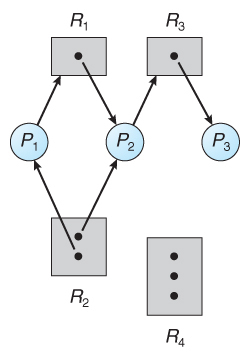
\includegraphics{./Drawings/EDAF35-Operating_Systems/Resource_Allocation_Graph.jpg}
  \caption{Resource Allocation Graph}
  \label{fig:Resource_Allocation_Graph}
\end{figure}

In \Cref{fig:Resource_Allocation_Graph}, there are:
\begin{itemize}[noitemsep]
\item The sets $P$, $R$, and $E$:
  \begin{itemize}[noitemsep]
  \item $P = \lbrace P_{1}, P_{2}, P_{3} \rbrace$
  \end{itemize}

\item Resource instances:
  \begin{itemize}[noitemsep]
  \item One instance of resource type $R_{1}$
  \item Two instances of resource type $R_{2}$
  \item One instance of resource type $R_{3}$
  \item Three instances of resource type $R_{4}$
  \end{itemize}

\item Process states:
  \begin{itemize}[noitemsep]
  \item Process $P_{1}$ is holding an instance of resource type $R_{2}$ and is waiting for an instance of resource type $R_{1}$.
  \item Process $P_{2}$ is holding an instance of $R_{1}$ and an instance of $R_{2}$ and is waiting for an instance of $R_{3}$.
  \item Process $P_{3}$ is holding an instance of $R_{3}$.
  \end{itemize}
\end{itemize}

Given the definition of a resource-allocation graph, if the graph contains no cycles, then no process in the system is \nameref{def:Deadlock}ed.
If the graph does contain a cycle, then a \nameref{def:Deadlock} may exist.
\begin{itemize}[noitemsep]
\item If each resource type has exactly one instance, then a cycle implies that a \nameref{def:Deadlock} has occurred.
  \begin{itemize}[noitemsep]
  \item In this case, a cycle in the graph is both a necessary and a sufficient condition for the existence of \nameref{def:Deadlock}.
  \end{itemize}
\item If each resource type has several instances, then a cycle does not necessarily imply that a \nameref{def:Deadlock} has occurred.
  \begin{itemize}[noitemsep]
  \item In this case, a cycle in the graph is a necessary but not a sufficient condition for the existence of \nameref{def:Deadlock}.
  \item This is illustrated by \Crefrange{subfig:Resource_Allocation_Graph-Cycle_Deadlock}{subfig:Resource_Allocation_Graph-Cycle_No_Deadlock}.
  \end{itemize}
\end{itemize}

\begin{figure}[h!tbp]
  \centering
  \begin{subfigure}[h!tbp]{0.48\linewidth}
    \centering
    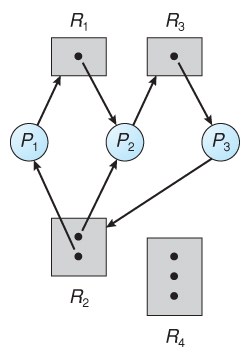
\includegraphics[scale=0.85]{./Drawings/EDAF35-Operating_Systems/Resource_Allocation_Graph-Deadlock.jpg}
    \caption{RAG with Cycle and Deadlock}
    \label{subfig:Resource_Allocation_Graph-Cycle_Deadlock}
  \end{subfigure}
  \begin{subfigure}[h!tbp]{0.48\linewidth}
    \centering
    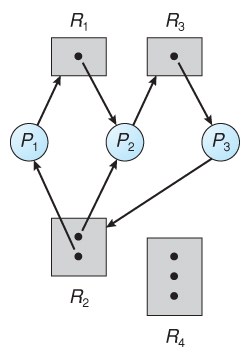
\includegraphics[scale=0.85]{./Drawings/EDAF35-Operating_Systems/Resource_Allocation_Graph-Cycle_No_Deadlock.jpg}
    \caption{RAG with Cycle but no Deadlock}
    \label{subfig:Resource_Allocation_Graph-Cycle_No_Deadlock}
  \end{subfigure}
  \caption{Resource Allocation Graph with Cycle}
  \label{fig:Resource_Allocation_Graph-Cycle}
\end{figure}

%%% Local Variables:
%%% mode: latex
%%% TeX-master: "../../EDAF35-Operating_Systems-Reference_Sheet"
%%% End:
